%https://github.com/SublimeText/LaTeXTools/issues/1439
%!TEX output_directory=latexcache

% You can build this using the command:
% latexmk -pdf -jobname=output -output-directory=cache -aux-directory=cache -pdflatex="pdflatex -interaction=nonstopmode" -use-make main.tex

% When the bibliography includes a cyclic reference to another bibliography,
% you need to run `pdflatex` 5 times on the following order:
% 1. `pdflatex`,
% 2. `biber`,
% 3. `pdflatex`
% 4. `pdflatex`
% 5. `pdflatex`
% 6. `biber`
% 7. `pdflatex`

% Monograph LaTeX Template for UFSC based on:
% 1. https://github.com/royertiago/tcc
% 2. http://portal.bu.ufsc.br/normalizacao/
% 3. https://github.com/evandrocoan/ufscthesisx
% 4. http://www.latextemplates.com/template/simple-sectioned-essay

% Initially translated from Portuguese with help of https://github.com/omegat-org/omegat <Computer Assisted Translation of LaTeX document>
% https://tex.stackexchange.com/questions/313732/computer-assisted-translation-of-latex-document

% Allows you to write your thesis both in English and Portuguese
% https://tex.stackexchange.com/questions/5076/is-it-possible-to-keep-my-translation-together-with-original-text
\newif\ifenglish\englishfalse
\newif\ifadvisor\advisorfalse

% Uncomment the line `\englishtrue` to set the document default language to English
% \englishtrue
\advisortrue

% https://tex.stackexchange.com/questions/131002/how-to-expand-ifthenelse-so-that-it-can-be-used-in-parshape
\newcommand{\lang}[2]{\ifenglish#1\else#2\fi}
\newcommand{\advisor}[2]{\ifadvisor#1\else#2\fi}

% https://tex.stackexchange.com/questions/385895/how-to-make-passoptionstopackage-add-the-option-as-the-last
% https://tex.stackexchange.com/questions/484400/changing-the-cleveref-package-language-conjunction-definition
% https://tex.stackexchange.com/questions/516058/why-isnt-my-biblatex-language-changing-when-passing-the-language-on-my-document
\ifenglish
    \PassOptionsToPackage{brazil,main=english,spanish,french}{babel}
\else
    \PassOptionsToPackage{main=brazil,english,spanish,french}{babel}
\fi

% Simple alias for English and Portuguese words
% https://tex.stackexchange.com/questions/513019/argument-of-bbltempd-has-an-extra
\newcommand{\brazilword}[1]{\protect\foreignlanguage{brazil}{#1}}
\newcommand{\englishword}[1]{\protect\foreignlanguage{english}{#1}}

% Allow you to write `Evandro's house` in latex as `Evandro\s house` instead of `Evandro\textquotesingle{}s house`
% https://tex.stackexchange.com/questions/31091/space-after-latex-commands
\newcommand{\s}[0]{\textquotesingle{}s\xspace}
\newcommand{\q}[0]{\textquotesingle{}\xspace}

% Uncomment the following line if you want to use other biblatex settings
% \PassOptionsToPackage{style=numeric,repeatfields=true,backend=biber,backref=true,citecounter=true}{biblatex}
\documentclass[
\lang{english}{brazilian,brazil}, % https://tex.stackexchange.com/questions/484400/changing-the-cleveref-package-language-conjunction-definition
12pt, % Padrão UFSC para versão final
a4paper, % Padrão UFSC para versão final
oneside, % Impressão nos dois lados da folha
chapter=TITLE, % Título de capítulos em caixa alta
section=TITLE, % Título de seções em caixa alta
]{setup/ufscthesisx}

% Utilize o arquivo aftertext/references.bib para incluir sua bibliografia.
% http://tug.ctan.org/tex-archive/macros/latex/contrib/cleveref/cleveref.pdf
\addbibresource{aftertext/references.bib}

% https://www.overleaf.com/learn/latex/Inserting_Images
\graphicspath{{pictures/}}

% FIXME: Preencha com seus dados
\autor{\brazilword{Gabriel Avila}}
\titulo{Geração Aumentada por Recuperação Aplicada à Interpretação de Metáforas Históricas: \\ Um Pipeline com LLMs e Evidências Textuais}

% FIXME: Se houver subtítulo, descomente a linha abaixo
% \subtitulo{\lang{Subtitle}{Subtítulo}}

% FIXME: Siglas para grau de formação Dr./Dra., Me./Ma, Bel. Bela. (inglês: PhD., MSc., Bs.)
\orientador[\lang{Supervisor}{Orientador(a)}]{\brazilword{Rodrigo Bragio Bonaldo}, \lang{Phd.}{Dr.}}

% FIXME: Se houver coorientador, descomente a linha abaixo
\coorientador[\lang{Responsible Professor}{Professor Responsável}]{\brazilword{Jean Carlo Rossa Hauck}, \lang{Phd.}{Dr.}}

% FIXME: Preencher com o nome do Coordenador de TCCs/Teses do seu curso
%\coordenador[\lang{Coordenador}{}]{\brazilword{Renato Cislaghi}, \lang{Phd.}{Dr.}}

% FIXME: Local da sua defesa
\local{\brazilword{Florianópolis, Santa Catarina} -- \lang{Brazil}{Brasil}}

% FIXME: Ano da sua defesa
\ano{2026}
\biblioteca{\lang{University Library}{Biblioteca Universitária}}

% FIXME: Sigla da sua instituição
\instituicaosigla{UFSC}
\instituicao{\brazilword{Universidade Federal de Santa Catarina}}

% FIXME: Preencha com Tese, Dissertação, Monografia ou Trabalho de Conclusão de Curso, Bachelor's Thesis, etc
\tipotrabalho{\lang{Bachelor\s Thesis}{Trabalho de Conclusão de Curso}}

% FIXME: Se houver Área de Concentração, descomente a linha abaixo
% \area{\lang{Formal Languages}{Linguagens Formais}}

% FIXME: Preencha com Doutor, Bacharel ou Mestrando
\formacao{\lang
    {Bachelor of Science degree in Information Systems}
    {Bacharel em Sistemas de Informação}%
}
\programa{\lang
    {Undergraduate Program in Information Systems}
    {Programa de Graduação em Sistemas de Informação}%
}

% FIXME: Preencha com Departamento de XXXXXX, Centro de XXXXXX
\centro{\lang
    {INE -- Department of Informatics and Statistics, CTC -- Technological Center}
    {INE -- Departamento de Informática e Estatística, CTC -- Centro Tecnológico}%
}

% FIXME: Preencha com Campus XXXXXX     ou     Centro de XXXXXX
\campus{\brazilword{Campus Reitor João David Ferreira Lima}}

% Data da entrega da proposta
\data{\lang{- of June of}{- de junho de} 2025}

% FIXME: Data da sua defesa
\data{\lang{- of december of}{- de dezembro de} 2026}

% O preambulo deve conter tipo do trabalho, objetivo, nome da instituição e a área de concentração.
\preambulo{\lang%
    {%
        \imprimirtipotrabalho~submitted to the \imprimirprograma~of
        \imprimirinstituicao~for degree acquirement in \imprimirformacao.%
    }{%
        \imprimirtipotrabalho~submetido ao \imprimirprograma~da
        \imprimirinstituicao~para a obtenção do Grau de \imprimirformacao.%
    }%
}

% Allows you to use ~= instead of `\hyp{}`
% https://tex.stackexchange.com/questions/488008/how-to-create-an-alternative-to-shortcut-or-hyp
% https://tex.stackexchange.com/questions/405718/depending-on-babel-language-setting-i-get-biblatex-error-argument-of-language
% https://tex.stackexchange.com/questions/340661/argument-of-languageactivearg-has-an-extra-i-use-includegraphics-and-r
\useshorthands{~}\defineshorthand{~=}{\hyp{}}

\palavraschaveufsc{palavraschaveingles}   {Natural Language Processing}
\palavraschaveufsc{palavraschaveportugues}{Processamento~=de~=Linguagem~=Natural}

\palavraschaveufsc{palavraschaveingles}   {Retrieval-Augmented Generation}
\palavraschaveufsc{palavraschaveportugues}{Geração~=Aumentada~=por~=Recuperação}

\palavraschaveufsc{palavraschaveingles}   {Large Language Models}
\palavraschaveufsc{palavraschaveportugues}{Grandes~=Modelos~=de~=Linguagem}

\palavraschaveufsc{palavraschaveingles}   {Metaphors}
\palavraschaveufsc{palavraschaveportugues}{Metáforas}

\palavraschaveufsc{palavraschaveingles}   {Diachronic Datasets}
\palavraschaveufsc{palavraschaveportugues}{Conjuntos~=de~=Dados~=Diacrônicos}

\palavraschaveufsc{palavraschaveingles}   {Semantic Change}
\palavraschaveufsc{palavraschaveportugues}{Mudança~=Semântica}

\palavraschaveufsc{palavraschaveingles}   {Temporal Corpora}
\palavraschaveufsc{palavraschaveportugues}{Corpora~=Temporais}

\palavraschaveufsc{palavraschaveingles}   {Historical Linguistics}
\palavraschaveufsc{palavraschaveportugues}{Linguística~=Histórica}

\hypersetup
{
    pdfsubject={Thesis' Abstract},
    pdfcreator={LaTeX with abnTeX2 for UFSC},
    pdftitle={\imprimirtitulo},
    pdfauthor={\imprimirautor},
    pdfkeywords={\lang{\palavraschaveinglessemitem}{\palavraschaveportuguessemitem}},
}

% Altere o arquivo 'settings.tex' para incluir customizações de aparência da sua tese
%----------------------------------------------------------------------------------------
%   Thesis Tweaks and Utilities
%----------------------------------------------------------------------------------------
\makeatletter


% Uncomment this if you are debugging pages' badness Underfull & Overflow
% https://tex.stackexchange.com/questions/115908/geometry-showframe-landscape
% https://tex.stackexchange.com/questions/387077/what-is-the-difference-between-usepackageshowframe-and-usepackageshowframe
% https://tex.stackexchange.com/questions/387257/how-to-do-the-memoir-headings-fix-but-not-have-my-text-going-over-the-page-botto
% https://tex.stackexchange.com/questions/14508/print-page-margins-of-a-document
% \usepackage[showframe,pass]{geometry}

% To use the font Times New Roman, instead of the default LaTeX font
% more up-to-date than '\usepackage{mathptmx}'
% \usepackage{newtxtext}
% \usepackage{newtxmath}

% https://tex.stackexchange.com/questions/182569/how-to-manually-set-where-a-word-is-split
\hyphenation{Ge-la-im}
\hyphenation{Cis-la-ghi}

% Add missing translations for Portuguese
% https://tex.stackexchange.com/questions/8564/what-is-the-right-way-to-redefine-macros-defined-by-babel
\@ifpackageloaded{babel}{\@ifpackagewith{babel}{brazil}{\addto\captionsbrazil{%
  \renewcommand{\mytextpreliminarylistname}{Breve Sumário}
}}{}}{}
\@ifundefined{advisor}{\newcommand{\advisor}[2]{#1}}{}

% Selects a sans serif font family
% \renewcommand{\sfdefault}{cmss}

% Selects a monospaced (“typewriter”) font family
% \renewcommand{\ttdefault}{cmtt}

% Spacing between lines and paragraphs
% https://tex.stackexchange.com/questions/70212/ifpackageloaded-question
\@ifclassloaded{memoir}
{
  % New custom chapter style VZ14, see other chapters styles in:
  % http://repositorios.cpai.unb.br/ctan/info/latex-samples/MemoirChapStyles/MemoirChapStyles.pdf
  \newcommand\thickhrulefill{\leavevmode \leaders \hrule height 1ex \hfill \kern \z@}
  \makechapterstyle{VZ14} { %
    % \thispagestyle{empty}
    \setlength\beforechapskip{50pt}
    \setlength\midchapskip{20pt}
    \setlength\afterchapskip{20pt}
    \renewcommand\chapternamenum{}
    \renewcommand\printchaptername{}
    \renewcommand\chapnamefont{\Huge\scshape}
    \renewcommand\printchapternum {%
      \chapnamefont\null\thickhrulefill\quad
      \@chapapp\space\thechapter\quad\thickhrulefill
    }
    \renewcommand\printchapternonum {%
      \par\thickhrulefill\par\vskip\midchapskip
      \hrule\vskip\midchapskip
    }
    \renewcommand\chaptitlefont{\huge\scshape\centering}
    \renewcommand\afterchapternum {%
      \par\nobreak\vskip\midchapskip\hrule\vskip\midchapskip
    }
    \renewcommand\afterchaptertitle {%
      \par\vskip\midchapskip\hrule\nobreak\vskip\afterchapskip
    }
  }

  % Apply the style `VZ14` just created
  % \chapterstyle{VZ14}

  % http://mirrors.ibiblio.org/CTAN/macros/latex/contrib/memoir/memman.pdf
  \setlength\beforechapskip{0pt}
  \setlength\midchapskip{15pt}
  \setlength\afterchapskip{15pt}

  % Memoir: Warnings “The material used in the headers is too large” w/ accented titles
  % https://tex.stackexchange.com/questions/387293/how-to-change-the-page-layout-with-memoir
  \setheadfoot{30.0pt}{\footskip}
  \checkandfixthelayout
}{}

% Controlling the spacing between one paragraph and another
% Default value for UFSC 0.0cm
\setlength{\parskip}{\advisor{0.0cm}{0.2cm}}

% Paragraph size is given by
% Default value for UFSC 1.5cm
% \setlength{\parindent}{1.3cm}

% https://tex.stackexchange.com/questions/148647/how-to-remove-space-before-enumerate
% https://tex.stackexchange.com/questions/433543/behaviour-of-enumitem-setlist
\advisor{}{
    \setlist*[enumerate]{label=\arabic*,}
    \setlist*[enumerateoptional]{label=\arabic*,}

    % https://tex.stackexchange.com/questions/24454/space-after-float-with-h
    % https://tex.stackexchange.com/questions/23313/how-can-i-reduce-padding-after-figure
    \AtBeginEnvironment{figure}{
      \setlength{\intextsep}{5pt} % Vertical space above & below [h] floats
      % \setlength{\textfloatsep}{10pt} % Vertical space below (above) [t] ([b]) floats
      % \setlength{\abovecaptionskip}{10pt}
      % \setlength{\belowcaptionskip}{5pt}
    }

    % Patch the `abntex2` citacao environment removing the extra space from its top
    % https://tex.stackexchange.com/questions/300340/topsep-itemsep-partopsep-and-parsep-what-does-each-of-them-mean-and-wha
    \xpatchcmd{\citacao}
    {\list{}}
    {\list{}{\topsep=0pt}}
    {}
    {\FAILEDPATCHINGCITACAO}
}


% Color settings across the document
\@ifpackageloaded{xcolor}
{
  % RGB colors in absolute values from 0 to 255 by using `RGB` tag
  \definecolor{darkblue}{RGB}{26,13,178}

  % Colors names definitions as RGB colors in percentage notation by using `rgb` tag
  \definecolor{mygreen}{rgb}{0,0.6,0}
  \definecolor{mygray}{rgb}{0.5,0.5,0.5}
  \definecolor{mymauve}{rgb}{0.58,0,0.82}
  \definecolor{figcolor}{rgb}{1,0.4,0}
  \definecolor{tabcolor}{rgb}{1,0.4,0}
  \definecolor{eqncolor}{rgb}{1,0.4,0}
  \definecolor{linkcolor}{rgb}{1,0.4,0}
  \definecolor{citecolor}{rgb}{1,0.4,0}
  \definecolor{seccolor}{rgb}{0,0,1}
  \definecolor{abscolor}{rgb}{0,0,1}
  \definecolor{titlecolor}{rgb}{0,0,1}
  \definecolor{biocolor}{rgb}{0,0,1}
  \definecolor{blue}{RGB}{41,5,195}

  % PDF Hyperlinks settings
  \@ifpackageloaded{hyperref}
  {
    \hypersetup
    {
      colorlinks=true,     % false: boxed links; true: colored links
      linkcolor=darkblue,  % color of internal links
      citecolor=darkblue, % color of links to bibliography
      filecolor=black,     % color of file links
      urlcolor=\advisor{black}{darkgreen},
      bookmarksdepth=4,
      pdfencoding=auto,%
      psdextra,
    }
  }
}{}


% Filtering and Mapping Bibliographies
% \DeclareFieldFormat{url}{Disponível~em:\addspace\url{#1}}

% https://tex.stackexchange.com/questions/517526/how-to-make-biblatex-url-links-generated-with-brackets-around-it-url-correctly
\DeclareFieldFormat{url}{\bibstring{urlfrom}\addcolon\space\textless\url{#1}\textgreater}
\DefineBibliographyStrings{brazil}{urlfrom = {Disponível em}}
\DefineBibliographyStrings{english}{urlfrom = {Available from}}

% https://tex.stackexchange.com/questions/391695/is-possible-to-remove-the-link-color-of-the-comma-on-the-citation-link
% \DeclareFieldFormat{citehyperref}{#1}

% % https://tex.stackexchange.com/questions/203764/reduce-font-size-of-bibliography-overfull-bibliography
% \newcommand{\bibliographyfontsize}{\fontsize{10.0pt}{10.5pt}\selectfont}
% \renewcommand*{\bibfont}{\bibliographyfontsize}

% Uncomment this to insert the abstract into your bibliography entries when the abstract is available
% https://tex.stackexchange.com/questions/398666/how-to-correctly-insert-and-justify-abstract
\ifadvisor
\else
  \DeclareFieldFormat{abstract}%
  {%
    \par\justifying
    \begin{adjustwidth}{1cm}{}
      \textbf{\bibsentence\bibstring{abstract}:} #1
    \end{adjustwidth}
  }
  \renewbibmacro*{finentry}%
  {%
    \iffieldundef{abstract}
    {\finentry}
    {\finentrypunct
      \printfield{abstract}%
      \renewcommand*{\finentrypunct}{}%
      \finentry
    }
  }

  % Backref package settings, pages with citations in bibliography
  \newcommand{\biblatexcitedntimes}{\autocap{c}ited \arabic{citecounter} times}
  \newcommand{\biblatexcitedonetime}{\autocap{c}ited one time}
  \newcommand{\biblatexcitednotimes}{\autocap{n}o citation in the text}

  \@ifpackageloaded{babel}{\@ifpackagewith{babel}{brazil}{\addto\captionsbrazil{%
    \renewcommand{\biblatexcitedntimes}{\autocap{c}itado \arabic{citecounter} vezes}
    \renewcommand{\biblatexcitedonetime}{\autocap{c}itado uma vez}
    \renewcommand{\biblatexcitednotimes}{\autocap{n}enhuma citação no texto}
  }}{}}{}
  \@ifpackageloaded{biblatex}
  {%
    % https://tex.stackexchange.com/questions/483707/how-to-detect-whether-the-option-citecounter-was-enabled-on-biblatex
    \ifx\blx@citecounter\relax
      \message{Is citecounter defined? NO!^^J}
    \else
      \message{Is citecounter defined? YES!^^J}
      \ifbacktracker
        \message{Is backtracker defined? YES!^^J}
        \renewbibmacro*{pageref}
        {%
          % https://tex.stackexchange.com/questions/516054/how-to-use-a-dot-to-separate-my-new-bibliography-entry
          \renewcommand*{\bibpagerefpunct}{\addperiod\space}%
          \iflistundef{pageref}%
          {\printtext{\biblatexcitednotimes}}
          {%
            \printtext
            {%
              \ifnumgreater{\value{citecounter}}{1}
                {\biblatexcitedntimes}
                {\biblatexcitedonetime}%
            }%
            \setunit{\addspace}%
            \ifnumgreater{\value{pageref}}{1}
              {\bibstring{backrefpages}\ppspace}
              {\bibstring{backrefpage}\ppspace}%
            \printlist[pageref][-\value{listtotal}]{pageref}%
          }%
        }

        \DefineBibliographyStrings{brazil}
        {
          backrefpage  = {na página},
          backrefpages = {nas páginas},
        }

        \DefineBibliographyStrings{english}
        {
          backrefpage  = {on page},
          backrefpages = {on pages},
        }
      \else
        \message{Is backtracker defined? NO!^^J}
      \fi
    \fi
  }{}
\fi


% https://tex.stackexchange.com/questions/516056/why-an-empty-or-not-biblatex-declaresourcemap-is-removing-my-bibliography-acces
% https://github.com/abntex/biblatex-abnt/pull/56/files
\DeclareStyleSourcemap{%% >>>2
  % This maps some fields used in abntex2cite to biblatex fields.
  \maps[datatype=bibtex]{%
    \map{%
      \step[fieldsource=conference-number,fieldtarget=number]%
      \step[fieldsource=conference-year,fieldtarget=eventdate]%
      \step[fieldsource=conference-location,fieldtarget=venue]%
      \step[fieldsource=conference-number,fieldtarget=number]%
      \step[fieldsource=org-short,fieldtarget=shortauthor]%
      \step[fieldsource=urlaccessdate,fieldtarget=urldate]%
      \step[fieldsource=year-presented,fieldtarget=eventyear]%
      \step[fieldsource=furtherresp,fieldtarget=titleaddon]%
      \step[typesource=journalpart,typetarget=supperiodical]%
    }%
    \map[overwrite=false]{%
      \step[fieldsource=reprinted-from, final]%
      \step[fieldset=related, origfieldval]%
    }%
    \map[overwrite=false]{%
      \step[fieldsource=reprinted-text, final]%
      \step[fieldset=relatedtype, fieldvalue={reprintfrom}]%
    }%
    \map{%
      \pertype{patent}% Use the organization as sourcekey for patents
      \step[fieldsource=organization, final]%
      \step[fieldset=sortkey, origfieldval]%
    }%
    \map[overwrite=false]{%
      \pertype{thesis}%
      \pertype{phdthesis}%
      \pertype{mastersthesis}%
      \pertype{monography}%
      \step[fieldset=bookpagination, fieldvalue={sheet}]%
    }%
    % remove fields that are always useless
    \map{
      % \step[fieldset=abstract, null]
      \step[fieldset=pagetotal, null]
    }
    % % remove URLs for types that are primarily printed
    % \map{
    %   \pernottype{software}
    %   \pernottype{online}
    %   \pernottype{report}
    %   \pernottype{techreport}
    %   \pernottype{standard}
    %   \pernottype{manual}
    %   \pernottype{misc}
    %   \step[fieldset=url, null]
    %   \step[fieldset=urldate, null]
    % }
    \map{
      \pertype{inproceedings}
      % remove mostly redundant conference information
      \step[fieldset=venue, null]
      \step[fieldset=eventdate, null]
      \step[fieldset=eventtitle, null]
      % do not show ISBN for proceedings
      \step[fieldset=isbn, null]
      % Citavi bug
      \step[fieldset=volume, null]
    }
  }%
}% <<<2


% https://tex.stackexchange.com/questions/14314/changing-the-font-of-the-numbers-in-the-toc-in-the-memoir-class
\renewcommand{\cftpartfont}{\ABNTEXpartfont\color{black}}
\renewcommand{\cftpartpagefont}{\ABNTEXpartfont\color{black}}

\renewcommand{\cftchapterfont}{\ABNTEXchapterfont\color{black}}
\renewcommand{\cftchapterpagefont}{\ABNTEXchapterfont\color{black}}

\renewcommand{\cftsectionfont}{\ABNTEXsectionfont\color{black}}
\renewcommand{\cftsectionpagefont}{\ABNTEXsectionfont\color{black}}

\renewcommand{\cftsubsectionfont}{\ABNTEXsubsectionfont\color{black}}
\renewcommand{\cftsubsectionpagefont}{\ABNTEXsubsectionfont\color{black}}

\renewcommand{\cftsubsubsectionfont}{\ABNTEXsubsubsectionfont\color{black}}
\renewcommand{\cftsubsubsectionpagefont}{\ABNTEXsubsubsectionfont\color{black}}

\renewcommand{\cftparagraphfont}{\ABNTEXsubsubsubsectionfont\color{black}}
\renewcommand{\cftparagraphpagefont}{\ABNTEXsubsubsubsectionfont\color{black}}

% Memoir has another mechanism for the job: \cftsetindents{‹kind›}{indent}{numwidth}. Here kind is
% chapter, section, or whatever; the indent specifies the ‘margin’ before the entry starts; and the
% width is of the box into which the number is typeset (so needs to be wide enough for the largest
% number, with the necessary spacing to separate it from what comes after it in the line.
% http://www.tex.ac.uk/FAQ-tocloftwrong.html
% https://tex.stackexchange.com/questions/264668/memoir-indentation-of-unnumbered-sections-in-table-of-contents
% https://tex.stackexchange.com/questions/394227/memoir-toc-indent-the-second-line-by-numberspace
%
% `\cftlastnumwidth` and these `\cftsetindents` are defined by the abntex2 class,
% obeying the `ABNTEXsumario-abnt-6027-2012`. \newlength{\cftlastnumwidth}
% \setlength{\cftlastnumwidth}{\cftsubsubsectionnumwidth}
% \addtolength{\cftlastnumwidth}{-1em}

% http://www.tex.ac.uk/FAQ-tocloftwrong.html
% Use \setlength\cftsectionnumwidth{4em} to override all these values at once
\ifadvisor
\else
  \makechapterstyle{fixedabntex2indentation}
  {%
    \renewcommand{\chapterheadstart}{}
    \setlength{\beforechapskip}{20pt}
    \setlength{\midchapskip}{20pt}
    \setlength{\afterchapskip}{15pt}

    \ifx \chapternamenumlength \undefined
      \newlength{\chapternamenumlength}
    \fi

    % tamanhos de fontes de chapter e part
    \ifthenelse{\equal{\ABNTEXisarticle}{true}}{%
      \setlength\beforechapskip{\baselineskip}%
      \renewcommand{\chaptitlefont}{\ABNTEXsectionfont\ABNTEXsectionfontsize}%
    }{%else
       \setlength{\beforechapskip}{0pt}%
       \renewcommand{\chaptitlefont}{\ABNTEXchapterfont\ABNTEXchapterfontsize}%
    }

    \renewcommand{\chapnumfont}{\chaptitlefont}
    \renewcommand{\parttitlefont}{\ABNTEXpartfont\ABNTEXpartfontsize}
    \renewcommand{\partnumfont}{\ABNTEXpartfont\ABNTEXpartfontsize}
    \renewcommand{\partnamefont}{\ABNTEXpartfont\ABNTEXpartfontsize}

    % tamanhos de fontes de section, subsection, subsubsection e subsubsubsection
    \setsecheadstyle{\ABNTEXsectionfont\ABNTEXsectionfontsize\ABNTEXsectionupperifneeded}
    \setsubsecheadstyle{\ABNTEXsubsectionfont\ABNTEXsubsectionfontsize\ABNTEXsubsectionupperifneeded}
    \setsubsubsecheadstyle{\ABNTEXsubsubsectionfont\ABNTEXsubsubsectionfontsize\ABNTEXsubsubsectionupperifneeded}
    \setsubsubsubsecheadstyle{\ABNTEXsubsubsubsectionfont\ABNTEXsubsubsubsectionfontsize\ABNTEXsubsubsubsectionupperifneeded}

    % Impressão do número do capítulo
    \renewcommand{\chapternamenum}{}

    % Impressão do nome do capítulo
    \renewcommand{\printchaptername}{%
       \chaptitlefont%
       \ifthenelse{\boolean{abntex@apendiceousecao}}{\appendixname}{}%
    }

    % Impressão do título do capítulo
    \def\printchaptertitle##1{%
      \chaptitlefont%
      \ifthenelse{\boolean{abntex@innonumchapter}}{\centering\ABNTEXchapterupperifneeded{##1}}{%
      \ifthenelse{\boolean{abntex@apendiceousecao}}{%
        \centering%
        \settowidth{\chapternamenumlength}{\printchaptername\printchapternum\afterchapternum}%
        \ABNTEXchapterupperifneeded{##1}%
      }{%
        \settowidth{\chapternamenumlength}{\printchaptername\printchapternum\afterchapternum}%
        \parbox[t]{\columnwidth-\chapternamenumlength}{\ABNTEXchapterupperifneeded{##1}}}%
      }%
    }

    % https://tex.stackexchange.com/questions/264668/memoir-indentation-of-unnumbered-sections-in-table-of-contents
    \renewcommand{\tocinnonumchapter}{%
      \addtocontents{toc}{\cftsetindents{chapter}{2.5em}{2em}}%
      \cftinserthook{toc}{A}}

    % Impressão do número do capítulo (no capítulo e não toc)
    \renewcommand{\printchapternum}{%
      \setboolean{abntex@innonumchapter}{false}%
      \chapnumfont%
      ~~\thechapter~%
      \ifthenelse{\boolean{abntex@apendiceousecao}}{%
        \tocinnonumchapter%
        ~\ABNTEXcaptiondelim~~%
      }{}%
    }

    \renewcommand{\ABNTEXcaptiondelim}{~\textendash~}
    \renewcommand{\afterchapternum}{}

    % Impressão do capítulo não numerado
    \renewcommand\printchapternonum{%
      \setboolean{abntex@innonumchapter}{true}%
    }
  }
  \chapterstyle{fixedabntex2indentation}

  \cftsetindents{part}          {0em} {3em}
  \cftsetindents{chapter}       {0em} {3em}
  \cftsetindents{section}       {0em} {4.3em}
  \cftsetindents{subsection}    {0em} {5.2em}
  \cftsetindents{subsubsection} {0em} {5.1em}
  \cftsetindents{paragraph}     {0em} {6.0em}
  \cftsetindents{subparagraph}  {0em} {7.0em}
\fi


\makeatother



% When writing a large document, it is sometimes useful to work on selected sections of the document
% to speed up compilation time: https://en.wikibooks.org/wiki/TeX/includeonly
\newif\ifforcedinclude\forcedincludefalse

% \addtoincludeonly{beforetext/agradecimentos}
% \addtoincludeonly{beforetext/epigrafe}
% \addtoincludeonly{beforetext/fichacatalografica}
% \addtoincludeonly{beforetext/folhadeaprovacao}
% \addtoincludeonly{beforetext/resumos}
% \addtoincludeonly{beforetext/siglas}
% \addtoincludeonly{beforetext/simbolos}

% Part 1
% \addtoincludeonly{chapters/introduction}
% \addtoincludeonly{chapters/motivation}
% \addtoincludeonly{chapters/beautifiers}

% Part 2
\addtoincludeonly{chapters/object_beautifier}
% \addtoincludeonly{chapters/conclusion}
% \addtoincludeonly{aftertext/aftertext}

% Control whether the full document will be generated
% Note: It will also generate severals errors like the following, which can be ignored
%       Latexmk: Missing input file: 'chapters/test.aux'
%
% You can make latex stop generate these errors, if you generate a full version
% of the document, before uncommenting these lines.
%
% Uncomment these two lines, to only partially generate the document
% \doincludeonly
% \forcedincludetrue


% https://tex.stackexchange.com/questions/85113/xrightarrow-text
\makeatletter
\newcommand{\xRightarrow}[2][]{\ext@arrow 0359\Rightarrowfill@{#1}{#2}}
\newcommand{\xLeftarrow}[2][]{\ext@arrow 0359\Leftarrowfill@{#1}{#2}}
\makeatother

% https://tex.stackexchange.com/questions/32208/footnote-runs-onto-second-page
\interfootnotelinepenalty=10000

% Disable the empty pages automatically put by memoir class, except the ones by \cleardoublepage
\ifforcedinclude\openany\else\fi

% https://tex.stackexchange.com/questions/171999/overfull-hbox-in-biblatex
% https://tex.stackexchange.com/questions/499457/why-my-document-is-not-hyphenation-on-words-starting-with-upper-case-letter-i
\emergencystretch=5em

% https://tex.stackexchange.com/questions/23313/how-can-i-reduce-padding-after-figure
% https://tex.stackexchange.com/questions/499580/how-to-keep-my-default-floating-environment-spacing-before-them-while-reducing
% \xpretocmd{\figure}{\setlength{\belowcaptionskip}{-10pt}}{}{}


\begin{document}
    % FIXME: Comment this after finishing the thesis, so you can start fixing the \flushbottom vs \raggedbottom
    % https://tex.stackexchange.com/questions/65355/flushbottom-vs-raggedbottom
    \raggedbottom

    % https://tex.stackexchange.com/questions/4705/double-space-between-sentences
    \frenchspacing

    % Uncomment this to put a ←← | ← (Go To Top/Go Back) on each section header
    \advisor{}{\addGoToSummary}

    % ELEMENTOS PRÉ-TEXTUAIS
    % Capa
\imprimircapa

% Folha de rosto
\imprimirfolhaderosto*{}

% Folha de aprovação
\addtotextpreliminarycontent{\lang{Approval Sheet}{Folha de Aprovação}}

\begin{folhadeaprovacao}

    \begin{center}
        {\imprimirautor}

        \vspace{1em}
        {\ABNTEXchapterfont\bfseries\MakeUppercase{\imprimirtitulo}%
        \ifnotempty{\imprimirsubtitulo}{: \imprimirsubtitulo}}

        \vspace{2em}
        \begin{minipage}{\textwidth}
            \lang{
                This \imprimirtipotrabalho~was presented to obtain the degree of \imprimirformacao%
                \ifnotempty{\imprimirarea}{, in the area of \imprimirarea} in the course \imprimirprograma.%
                Approved on \imprimirdata.
            }{
                Este(a) \imprimirtipotrabalho~foi apresentado(a) para obtenção do título de \imprimirformacao%
                \ifnotempty{\imprimirarea}{, na área de concentração de \imprimirarea} no curso de \imprimirprograma.%
                Aprovado em \imprimirdata.
            }
        \end{minipage}
    \end{center}

    \vspace{2em}

    % Only show if coordinator is different from advisor
    \ifthenelse{\equal{\imprimircoordenador}{\imprimirorientador}}{}{%
        \assinatura{
            \textbf{\imprimircoordenador} \\
            \lang{Supervisor professor}{Professor responsável pelo trabalho}
        }
    }

    \assinatura{
        \textbf{\imprimirorientador} \\
        \imprimirorientadorRotulo
    }

    \ifnotempty{\imprimircoorientador}{%
        \assinatura{
            \textbf{\imprimircoorientador} \\
            \imprimircoorientadorRotulo
        }
    }

\end{folhadeaprovacao}
\vspace*{1cm}
\noindent
{\Large\bfseries Avaliação da Proposta de TCC\par}
\vspace{0.5cm}

\small
\noindent
\textbf{Instruções para preenchimento pelo \underline{orientador do trabalho}:}\\
Para cada critério avaliado, assinale um X na coluna “Sim” apenas se considerado aprovado.
Caso contrário, indique as alterações necessárias na coluna “Observação”.

\vspace{0.5cm}
\begin{tabularx}{\textwidth}{|p{0.45\textwidth}|
                                >{\centering\arraybackslash}p{0.07\textwidth}|
                                >{\centering\arraybackslash}p{0.07\textwidth}|
                                >{\centering\arraybackslash}p{0.07\textwidth}|
                                >{\centering\arraybackslash}p{0.07\textwidth}|
                                X|}
  \hline
  \textbf{Critérios} & \textbf{Sim} & \textbf{Parcial} & \textbf{Não} & \textbf{N/A} & \textbf{Observação} \\
  \hline
  1. O trabalho é adequado para um TCC no CCO/SIN (relevância / abrangência)? & & & & & \\
  \hline
  2. O título do trabalho é adequado? & & & & & \\
  \hline
  3. O tema de pesquisa está claramente descrito? & & & & & \\
  \hline
  4. O problema/hipóteses estão identificados? & & & & & \\
  \hline
  5. A relevância da pesquisa é justificada? & & & & & \\
  \hline
  6. Os objetivos descrevem claramente o que se pretende alcançar? & & & & & \\
  \hline
  7. O método proposto é adequado aos objetivos? & & & & & \\
  \hline
  8. O cronograma é coerente? & & & & & \\
  \hline
  9. Custos identificados (se houver) e financiamento previstos? & & & & & \\
  \hline
  10. Todas as pessoas envolvidas foram identificadas? & & & & & \\
  \hline
  11. Formas de comunicação definidas? & & & & & \\
  \hline
  12. Riscos potenciais identificados? & & & & & \\
  \hline
  13. Caso envolva software/empresa, há declaração (Anexo 3) de ciência? & & & & & \\
  \hline
\end{tabularx}

\vspace{1cm}

% Avaliação final
\noindent
\begin{tabularx}{\textwidth}{|X|X|}
  \hline
  \textbf{Avaliação Final} & $\Box$ Aprovado \quad\quad $\Box$ Não Aprovado \\
  \hline
  \textbf{Professor Responsável} & (Nome)\hfill(Data)\hfill(Assinatura) \\
  \hline
  \textbf{Orientador Externo (se houver)} & (Nome)\hfill(Data)\hfill(Assinatura) \\
  \hline
\end{tabularx}


% Resumo
% Portuguese Abstract
\cleardoublepage\phantomsection
\addtotextpreliminarycontent{Resumo}
\begin{otherlanguage*}{brazil}
\begin{resumo}[Resumo]
    A classificação automática de metáforas em contextos históricos representa um desafio relevante no campo do Processamento de Linguagem Natural (PLN), dada a natureza subjetiva, contextual e evolutiva das expressões metafóricas. Enquanto a maior parte dos trabalhos em PLN concentra-se na detecção de metáforas (classificação binária), este projeto parte de um pipeline onde metáforas já foram previamente identificadas, com o objetivo de classificá-las em categorias históricas específicas baseadas no referencial de Fernández Sebastián (2024). Ao fazê-lo, o projeto visa colaborar com a construção e expansão de um dataset diacrônico voltado à análise interpretativa de metáforas políticas e sociais em fontes textuais históricas. O trabalho é dividido em dois módulos principais. O primeiro, denominado \textit{Metaphor Classifier}, realiza a classificação das metáforas detectadas e expande o corpus por meio da recuperação de ocorrências semanticamente similares em obras históricas vetorizadas. Já o segundo módulo, baseado no paradigma \textit{Retrieval-Augmented Generation} (RAG), é responsável por gerar justificativas textuais embasadas para cada classificação atribuída, citando trechos das fontes históricas como evidência e articulando-os conceitualmente às categorias históricas definidas. A metodologia adota uma abordagem mista. A dimensão quantitativa será aplicada na avaliação de classificações automatizadas (via métricas como \textit{precision}, \textit{recall} e \textit{F1-score}, quando pertinente), enquanto a dimensão qualitativa garantirá a coerência conceitual dos pares gerados (\textit{metáfora, evidência, categoria}), com apoio de uma equipe interdisciplinar de historiadores. Como resultados esperados, prevê-se a entrega de um pipeline funcional e documentado capaz de gerar pelo menos 100 pares validados de metáforas com evidências e classificações históricas, além de justificativas explicativas geradas via LLMs. Este recurso poderá servir de base empírica para estudos historiográficos e fomentar novas hipóteses sobre o uso e transformação de metáforas no discurso político e social ao longo do tempo. O projeto contribui, assim, não apenas com a inovação metodológica na interseção entre história e PLN, mas também com a promoção de maior transparência e rastreabilidade na interpretação automatizada de linguagem metafórica.

    \imprimirpalavraschave{Palavras-chave}{\begin{inparaitem}[]\palavraschaveportugues\end{inparaitem}}
\end{resumo}
\end{otherlanguage*}

% English Abstract
\cleardoublepage\phantomsection
\addtotextpreliminarycontent{Abstract}
\begin{otherlanguage*}{english}
\begin{resumo}[Abstract]
    The automatic classification of metaphors in historical contexts poses a significant challenge in the field of Natural Language Processing (NLP), due to the subjective, contextual, and evolving nature of metaphorical expressions. While most NLP work focuses on metaphor detection (binary classification), this project begins from a pipeline in which metaphors have already been identified, with the goal of classifying them into specific historical categories based on the framework proposed by Fernández Sebastián (2024). In doing so, the project aims to support the construction and expansion of a diachronic dataset focused on the interpretive analysis of political and social metaphors in historical textual sources.

    The work is divided into two main modules. The first, called the \textit{Metaphor Classifier}, performs the classification of detected metaphors and expands the corpus by retrieving semantically similar occurrences in vectorized historical works. The second module, based on the \textit{Retrieval-Augmented Generation} (RAG) paradigm, is responsible for generating textual justifications for each assigned classification, quoting excerpts from historical sources as evidence and conceptually linking them to the defined historical categories.

    The methodology follows a mixed approach. The quantitative dimension will be applied in the evaluation of automated classifications (using metrics such as \textit{precision}, \textit{recall}, and \textit{F1-score}, where applicable), while the qualitative dimension will ensure the conceptual coherence of the generated triplets (\textit{metaphor, evidence, category}), with support from an interdisciplinary team of historians. The project also adopts principles of modular and iterative development, allowing flexibility in adapting to data and tools delivered by other members of the research group.

    As expected outcomes, the project aims to deliver a functional and documented pipeline capable of producing at least 100 validated metaphor pairs with historical classifications and supporting justifications generated via LLMs. This resource may serve as an empirical foundation for historiographical studies and stimulate new hypotheses about the use and transformation of metaphors in political and social discourse over time. The project thus contributes not only to methodological innovation at the intersection of history and NLP, but also to promoting greater transparency and traceability in the automated interpretation of metaphorical language.

    \imprimirpalavraschave{Keywords}{\begin{inparaitem}[]\palavraschaveingles\end{inparaitem}}
\end{resumo}
\end{otherlanguage*}


% Lista de abreviaturas e siglas
\addtotextpreliminarycontent{\lang{List of Acronyms}{Lista de Siglas}}

\begin{siglas}
    \item[PLN] \lang{Natural Language Processing}{Processamento de Linguagem Natural}
    \item[RAG] \lang{Retrieval-Augmented Generation}{Geração Aumentada por Recuperação}
    \item[LLM] \lang{Large Language Model}{Modelo de Linguagem de Grande Escala}
    \item[PoC] \lang{Proof of Concept}{Prova de Conceito}
    \item[K-NN] \lang{K-Nearest Neighbors algorithm}{Algoritmo dos K Vizinhos Mais Próximos}
    \item[TCC] \lang{Bachelor's Thesis}{Trabalho de Conclusão de Curso}
    \item[UFSC] \lang{Federal University of Santa Catarina}{Universidade Federal de Santa Catarina}
    \item[VLab] \lang{Virtual Laboratory (UFSC)}{Laboratório Virtual da UFSC}
\end{siglas}

\addtotextpreliminarycontent{\lang{List of Symbols}{Lista de Símbolos}}

% Devem aparecer na mesma ordem de ocorrência no texto.
\begin{simbolos}
    \item[$\rightarrow$] \lang{Relation or mapping (e.g., metaphor $\rightarrow$ evidence)}{Relação ou mapeamento (ex.: metáfora $\rightarrow$ evidência)}
    \item[$\ge$] \lang{Greater than or equal to}{Maior ou igual que}
    \item[*F1-score*] \lang{Harmonic mean between precision and recall}{Média harmônica entre precisão e revocação}
    \item[*precision*] \lang{Proportion of relevant items among retrieved ones}{Proporção de itens relevantes entre os recuperados}
    \item[*recall*] \lang{Proportion of relevant items retrieved from all available ones}{Proporção de itens relevantes recuperados entre os disponíveis}
\end{simbolos}

\cleardoublepage
\listoffigures
\cleardoublepage
\listoftables

% Sumário
\cleardoublepage
\hypersetup{hidelinks}
\addtotextpreliminarycontent{\contentsname}
\tableofcontents



    % ELEMENTOS TEXTUAIS
    \textual
    \setlength\beforechapskip{50pt}
    \setlength\midchapskip{20pt}
    \setlength\afterchapskip{20pt}

    % PROPOSTA DE TCC
    \providecommand{\tightlist}{}
\chapter{Proposta}
\section{\textbf{Introdução}}{Introdução}\label{introduuxe7uxe3o}

A classificação automática de metáforas constitui um desafio clássico no
campo do processamento de linguagem natural (PLN), devido à natureza
abstrata e dependente de contexto das expressões metafóricas.
Diferentemente das abordagens tradicionais que buscam identificar a
presença ou ausência de metáforas, este trabalho recebe metáforas já
detectadas em um pipeline prévio e propõe classificá-las em categorias
específicas baseadas no referencial histórico proposto por Fernández
Sebastián (2024). Esta classificação, sustentada teoricamente pelo
estudo qualitativo e erudito das fontes históricas, visa compreender
mais profundamente os padrões e o desenvolvimento das metáforas ao longo
do tempo. Essa tarefa ocorre no contexto da construção de um dataset
diacrônico --- um recurso ainda relativamente raro em PLN --- cuja
curadoria está sendo conduzida por outros membros da equipe. O presente
trabalho contribui com sua expansão e validação por meio da
classificação automatizada das metáforas e da recuperação de evidências
históricas.

Além disso, o projeto contempla dois módulos complementares: o
\emph{Metaphor Classifier}, que classifica e expande o conjunto de
metáforas por meio da recuperação de trechos semanticamente semelhantes
nas fontes históricas; e o \emph{RAG} (Retrieval-Augmented Generation),
responsável por gerar justificativas textuais embasadas, citando
passagens das obras consultadas. Este segundo módulo combina capacidades
avançadas dos modelos grandes de linguagem (LLMs) com mecanismos de
recuperação automatizada de contextos históricos e literários
relevantes. Espera-se, assim, contribuir para uma compreensão mais
fundamentada e transparente de metáforas em corpora históricos,
oferecendo suporte empírico para hipóteses historiográficas. O RAG cumpre 
a função central do trabalho de prova historiográfico, atuando em sua 
função referencial \citep{lewis2020retrieval}.

\section{\textbf{Objetivos}}{Objetivos}\label{objetivos}

\subsection{\texorpdfstring{\textbf{Objetivo
Geral}}{Objetivo Geral}}\label{objetivo-geral}

Desenvolver e integrar dois módulos: o \emph{Metaphor Classifier},
responsável por atribuir categorias históricas a metáforas previamente
detectadas e expandir o conjunto de exemplos por meio de recuperação
semântica de ocorrências análogas; e o \emph{RAG}, voltado à geração de
justificativas textuais embasadas, citando e recuperando evidências 
históricas relevantes para cada classificação.

\subsection{\texorpdfstring{\textbf{Objetivos
Específicos}}{Objetivos Específicos}}\label{objetivos-especuxedficos}

\begin{enumerate}
\def\labelenumi{\arabic{enumi}.}
\item
  \textbf{Construção de regras de categorização}\\
  Desenvolver regras interpretáveis com base em um documento de
  categorias e exemplos elaborado por historiadores, de modo a
  possibilitar a atribuição automática ou semi-automática de categorias
  históricas a metáforas detectadas.
\item
  \textbf{Metaphor Classifier --- Recuperação de evidências
  históricas}\\
  Dado um conjunto de metáforas detectadas, atribua categorias
  históricas e recupere metáforas similares em contextos históricos,
  compondo pares metáfora~$\leftrightarrow$~evidência textual.
\item
  \textbf{RAG --- Geração de justificativas explicativas}\\
  Desenvolver um segundo módulo capaz de gerar respostas textuais
  explicativas para cada metáfora classificada, citando a evidência
  textual recuperada e a justificando com base na categoria histórica
  atribuída.
\item
  \textbf{Avaliação funcional do pipeline}\\
  Avaliando-os com métricas formais (como F1-score ou precisão, se
  aplicável) ou, se simbólicos, com checklist qualitativo.
\item
  \textbf{Documentação e replicabilidade prática}\\
  Manter documentação clara e progressiva no repositório do projeto,
  incluindo instruções de uso, descrição das etapas e exemplos de
  entrada e saída para cada módulo.
\item
  \textbf{Flexibilidade de escopo e adaptação contínua}\\
  Conduzir o desenvolvimento sob abordagem iterativa e adaptativa,
  permitindo ajustes de rota conforme os dados e insumos forem
  disponibilizados por terceiros, respeitando os marcos definidos no
  cronograma.
\end{enumerate}

\subsection{Escopo do Trabalho}\label{escopo-do-trabalho}

\subsubsection{1 · Entradas externas
(pré-requisitos)}\label{entradas-externas-pruxe9-requisitos}

\begin{table}[htbp]
  \small
  \caption{Entradas externas (pré-requisitos)}    % Tabela 1
  \label{tab:entradas}
  \centering
  \begin{tabularx}{\linewidth}{@{}>{\RaggedRight\arraybackslash}p{2.5cm}
                                    >{\RaggedRight\arraybackslash}X
                                    >{\centering\arraybackslash}p{2.2cm}
                                    >{\RaggedRight\arraybackslash}p{2.4cm}
                                    >{\RaggedRight\arraybackslash}p{3.3cm}@{}}
    \toprule
    Origem & Entregável & Data prevista & Formato & Observação \\ \midrule
    Eduardo   & Embeddings vetoriais das obras históricas & 31 jul 2025 & Parquet / FAISS / Chroma & Recuperação semântica \\[2pt]
    Franciele & Documento de categorias (3 exemplos cada) & 15 ago 2025 & Markdown & Base p/ regras de categorização \\
    \bottomrule
  \end{tabularx}
  \fonte{Elaboração própria.}
\end{table}

\subsubsection{2 · Contribuições diretas do
autor}\label{contribuiuxe7uxf5es-diretas-do-autor}

\begin{table}[htbp]
  \small
  \caption{Contribuições diretas do autor}        % Tabela 2
  \label{tab:contribuicoes}
  \centering
  \begin{tabularx}{\linewidth}{@{}>{\RaggedRight\arraybackslash}p{3cm}
                                    >{\RaggedRight\arraybackslash}X
                                    >{\RaggedRight\arraybackslash}p{4.2cm}@{}}
    \toprule
    Módulo & Descrição resumida & Critério de aceite \\ \midrule
    \textbf{Metaphor Classifier} & Classifica metáforas detectadas e recupera expressões análogas em obras históricas. & $\geq$ 100 pares \textit{(metáfora, evidência, categoria)} gerados; execução end-to-end comprovada \\[2pt]
    \textbf{QuantEval} & Avalia a qualidade e coerência dos pares por checklist ou métricas formais. & Relatório técnico em Markdown com amostra comentada ou validação formal \\[2pt]
    \textbf{RAG} & Gera justificativas textuais baseadas na evidência recuperada. & Executável em $\geq$ 10 metáforas distintas com justificativas coerentes e citação da fonte \\
    \textbf{Docs} & Documentação viva (README, exemplos, instruções) atualizada a cada entrega. & Cada etapa entregue contém documentação correspondente no repositório \\ \bottomrule
  \end{tabularx}
  \fonte{Elaboração própria.}
\end{table}


\subsubsection{3 · Fora do escopo}\label{fora-do-escopo}

\begin{itemize}
\tightlist
\item
  Detecção inicial de metáforas (Classificação Binária)
\item
  Dataset-A (pré-existente)\\
\item
  OCR, interface web\\
\item
  LLM fine-tuned usada no RAG (fornecida por terceiros)
\end{itemize}

\subsubsection{4 · Premissas \&
restrições}\label{premissas-restriuxe7uxf5es}

\begin{itemize}
\tightlist
\item
  VLab-UFSC disponível com GPU/CPU até \textbf{julho/2026}.\\
\item
  Textos históricos em domínio público; nenhuma licença adicional é
  necessária.\\
\item
  Volume de dados modesto (\textless{} 10 GB); notebook pessoal e Google
  Drive são suficientes como redundância.\\
\item
  Se embeddings ou categorias atrasarem, o escopo será reduzido ou o
  autor assumirá tarefas extras.
\end{itemize}

\subsubsection{5 · Cronograma técnico
resumido}\label{cronograma-tuxe9cnico-resumido}

\begin{itemize}
\tightlist
\item
  \textbf{mar--abr 2025}

  \begin{itemize}
  \tightlist
  \item
    Leitura de fundamentos sobre RAG
  \item
    PoC inicial com prompt fixo
  \item
    Leitura dos capítulos 4--7 de Fernández Sebastián
  \item
    Estudo do estado da arte sobre PLN e metáforas
  \item
    Base estruturada inicial do \emph{Metaphor Classifier}
  \end{itemize}
\item
  \textbf{jul--ago 2025}

  \begin{itemize}
  \tightlist
  \item
    Recebimento dos embeddings (Eduardo)
  \item
    Recebimento do documento de categorias (Franciele)
  \item
    Implementação do \emph{Metaphor Classifier}
  \end{itemize}
\item
  \textbf{set--out 2025}

  \begin{itemize}
  \tightlist
  \item
    Expansão do Dataset-B com recuperação de metáforas similares
  \item
    Ajuste das regras de categorização com base nas novas evidências
  \item
    Avaliação funcional do \emph{Metaphor Classifier} (QuantEval)
  \item
    Desenvolvimento do módulo \emph{RAG} (geração de justificativas
    textuais)
  \item
    Redação do Projeto II
  \end{itemize}
\item
  \textbf{dez 2025 -- fev 2026}

  \begin{itemize}
  \tightlist
  \item
    Curadoria de logs e análise de falhas
  \item
    Organização de outputs e documentação técnica
  \item
    Planejamento da redação final do TCC
  \end{itemize}
\item
  \textbf{mar--jun 2026}

  \begin{itemize}
  \tightlist
  \item
    Versão revisada(foco em precisão) dos Scripts
  \item
    Redação da versão completa do TCC final
  \end{itemize}
\item
  \textbf{jun 2026}

  \begin{itemize}
  \tightlist
  \item
    Margem para retorno da banca antes da defesa
  \item
    Preparação da defesa pública (slides, ensaios)
  \end{itemize}
\item
  \textbf{jul 2026}

  \begin{itemize}
  \tightlist
  \item
    Ajustes finais e formatação ABNT
  \item
    Depósito do TCC na BU/UFSC
  \end{itemize}
\end{itemize}

\section{\textbf{Método de Pesquisa}}{Método de Pesquisa}\label{muxe9todo-de-pesquisa}

Adotar-se-á uma abordagem mista, combinando métodos quantitativos e
qualitativos. A dimensão \textbf{quantitativa} será utilizada sempre que
o processo de classificação empregar modelos supervisionados, com
aplicação de métricas como \emph{F1-score}, \emph{precision} e
cobertura. Caso o classificador opere de forma simbólica, a avaliação
seguirá uma abordagem qualitativa baseada em checklist, com inspeção
manual da correspondência entre metáfora, categoria atribuída e
evidência textual recuperada.

A dimensão \textbf{qualitativa} estará presente tanto na definição das
categorias quanto na validação da coerência histórico-conceitual dos
pares gerados (\emph{metáfora~$\leftrightarrow$~evidência}). Nessa etapa, as
classificações e justificativas produzidas pelos módulos serão
analisadas à luz do referencial de Fernández Sebastián, com apoio da
equipe de historiadores do projeto.

Trata-se de um estudo descritivo-exploratório, cujo objetivo principal é
mapear e caracterizar padrões metafóricos diacrônicos com base em fontes
textuais históricas. Não se busca inicialmente estabelecer relações de
causalidade, mas sim levantar regularidades e hipóteses interpretativas
que possam ser testadas posteriormente em estudos historiográficos mais
amplos.

A pesquisa é de natureza aplicada, voltada ao desenvolvimento de módulos
computacionais que integrarão um pipeline mais amplo. Dentre esses
módulos, destacam-se o \emph{Metaphor Classifier}, responsável pela
categorização e expansão do conjunto de metáforas, e o \emph{RAG},
voltado à geração textual explicativa com embasamento rastreável.

Serão utilizadas técnicas modernas de PLN, como \emph{Large Language
Models} (LLMs), vetorização semântica e algoritmos de vizinhança (K-NN).
As ferramentas específicas --- como bibliotecas de vetorização, índices
semânticos ou modelos de geração --- serão escolhidas conforme os
requisitos práticos da implementação.

A execução ocorrerá em ambiente computacional misto, utilizando notebook
pessoal e infraestrutura da UFSC, como o
\href{https://jupyter.vlab.ufsc.br/hub}{VLab da UFSC}, bem como o
repositório colaborativo
\href{https://github.com/iaehistoriaUFSC/metaphoriq}{IAeHistoriaUFSC},
no qual o progresso do projeto será mantido de forma incremental e
documentada.

\section{\textbf{Cronograma}}{Cronograma}\label{cronograma}

\begin{quote}
\textbf{Nota:} O cronograma abaixo parte do pressuposto de que certos
insumos técnicos --- como embeddings vetoriais das obras históricas e
etapas de pré-processamento --- estão sendo desenvolvidos paralelamente
por integrantes da equipe técnica (especialmente Maiko Nunes, Giovanna
Ramalho e Eduardo Goulart). O autor assume a integração desses artefatos
nos módulos sob sua responsabilidade, sem duplicar esforços já em curso.
\end{quote}

\begin{figure}[H]
  \centering
  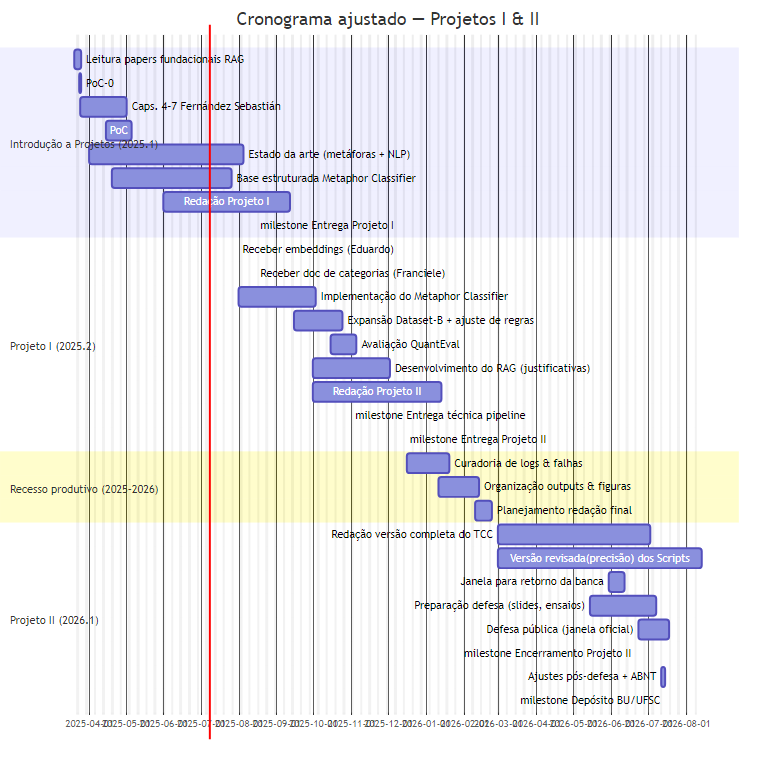
\includegraphics[height=0.7\textheight,keepaspectratio]{pictures/gantt.png}
  \caption{Diagrama de Gantt}
  \label{fig:gantt}
\end{figure}

\section{\textbf{Custos}}{Custos}\label{custos}

Não há custos previstos para a execução deste trabalho, uma vez que
todos os recursos necessários --- incluindo ferramentas de processamento
de linguagem natural, repositórios digitais, infraestrutura
computacional (como o VLab da UFSC) e canais de comunicação --- são
gratuitos, institucionais ou já disponíveis para os membros da equipe.

\section{\textbf{Recursos
Humanos}}{Recursos Humanos}\label{recursos-humanos}

\begin{table}[htbp]
  \small
  \caption{Recursos humanos envolvidos}           % Tabela 3
  \label{tab:rh}
  \centering
  \begin{tabularx}{\linewidth}{@{}>{\RaggedRight\arraybackslash}p{5.5cm}
                                    >{\RaggedRight\arraybackslash}X@{}}
    \toprule
    Nome & Função \\ \midrule
    Rodrigo Bragio Bonaldo & Orientador \\
    Jean Carlo Rossa Hauck & Coorientador/Responsável \\
    Chiru Stefan & Mentor técnico \\
    Patricia Biral Varela & Pesquisadora em História (aprendiz técnica) \\
    Maiko Ademir Nunes & Desenvolvedor Junior \\
    Giovanna Ramalho & Engenharia de Software \\
    Eduardo Peres Luckner Goulart & Desenvolvedor Junior \\
    Franciele Dias da Silva & Pesquisadora em História com função
    organizacional \\
    Mateus Freitas Borsatti & Pesquisador em História \\
    Letícia Portella Milan & Pesquisadora em História \\
    Éric Gabriel Kundlatsch & Pesquisador em História \\
    Isabella Stersa de Oliveira & Pesquisadora em História \\
    Gilson Mateus Pinto Júnior & Pesquisador em História \\
    Leonardo Nogueira Aucar & Pesquisador em História \\
    Gabriela Graudenz Muller & Linguística \\
    Willian Meurer Welter & Pesquisador em História \\
    Danillo Melo da Fonseca & Pesquisador em História (aprendiz técnico) \\
    Alysson Julio Risso da Silva & Pesquisador em História \\
    Marcel Vieira Silva & Pesquisador em História (aprendiz técnico) \\
    Thamiris Fátima dos Santos & Desenvolvedor Front-End \\
    Renata da Conceição Aquino da Silva & Pesquisadora em História \\
    Fernanda Lyrio Heinzelmann & Psicologia \\
    Breno Ampáro & Pesquisador em História \\
    Gabriel Choucair Garcia & Pesquisador em História \\ \bottomrule
  \end{tabularx}
  \fonte{Elaboração própria.}
\end{table}

\section{\textbf{Comunicação}}{Comunicação}\label{comunicauxe7uxe3o}

\begin{table}[htbp]
  \small
  \caption{Plano de comunicação}                  % Tabela 4
  \label{tab:comunicacao}
  \centering
  \begin{tabularx}{\linewidth}{@{}>{\RaggedRight\arraybackslash}p{4.8cm}
                                    >{\RaggedRight\arraybackslash}p{1.6cm}
                                    >{\RaggedRight\arraybackslash}p{2.4cm}
                                    >{\RaggedRight\arraybackslash}p{2.8cm}
                                    >{\RaggedRight\arraybackslash}X@{}}
    \toprule
    O que será comunicado & Por quem & Para quem & Meio & Frequência \\ \midrule
    Progresso técnico (pipeline, classificador, RAG) & Autor & Equipe técnica & Reunião Google Meet & Ter 14 h - 16 h semanal \\[2pt]
    Discussões conceituais sobre categorias & Autor & Equipe de História & Reunião Google Meet & Ter 16h30 - 17h30 semanal \\[2pt]
    Dúvidas de código/ferramentas & Autor & Stefan (coorientador técnico) & WhatsApp ou reunião & Sob demanda / semanal \\[2pt]
    Entregas parciais & Autor & Orientador(es) & GitHub / reunião & Ao final de cada etapa \\[2pt]
    Integrações entre módulos & Equipe técnica & Integrador designado & WhatsApp / Discord & Quando necessário \\[2pt]
    Avisos gerais & Autor & Todos & Grupo “IA e História” (WhatsApp) & Assíncrono contínuo \\ \bottomrule
  \end{tabularx}
  \fonte{Elaboração própria.}
\end{table}

\section{\textbf{Riscos}}{Riscos}\label{riscos}

\begin{table}[htbp]
  \small
  \caption{Riscos potenciais do projeto}          % Tabela 5
  \label{tab:riscos}
  \centering
  \begin{tabularx}{\linewidth}{@{}>{\RaggedRight\arraybackslash}p{4.2cm}
                                    >{\centering\arraybackslash}p{1.9cm}
                                    >{\centering\arraybackslash}p{1.5cm}
                                    >{\centering\arraybackslash}p{1.6cm}
                                    >{\RaggedRight\arraybackslash}p{3.1cm}
                                    >{\RaggedRight\arraybackslash}X@{}}
    \toprule
    Risco & Probabilidade & Impacto & Prioridade & Estratégia de resposta & Ações de prevenção \\ \midrule
    Integração complexa entre etapas do pipeline & Baixa & Alta & Média & Modularizar componentes & Revisões técnicas semanais com Stefan \\[2pt]
    Ingestão do dataset diacrônico demanda maior esforço & Alta & Alta & Alta & Reduzir escopo ou redefinir metas & Pilotos incrementais e testes de carga \\ \bottomrule
  \end{tabularx}
  \fonte{Elaboração própria.}
\end{table}
  

    % PARTE

    % PARTE

    % Segundo capitulo de Resultados

    % Finaliza a parte no bookmark do PDF para que se inicie o bookmark na raiz
    % e adiciona espaço de parte no Sumário
    \phantompart

    % Conclusão (outro exemplo de capítulo sem numeração e presente no sumário)

    % ELEMENTOS PÓS-TEXTUAIS
    \postextual
    \setlength\beforechapskip{0pt}
    \setlength\midchapskip{15pt}
    \setlength\afterchapskip{15pt}

    % Referências bibliográficas
    \begingroup
        % https://tex.stackexchange.com/questions/163559/how-to-modify-line-spacing-per-entry-of-bibliography
        % https://tex.stackexchange.com/questions/19105/how-can-i-put-more-space-between-bibliography-entries-biblatex
        \setlength\bibitemsep{\baselineskip}
        \advisor{}{\linespread{1.18}\selectfont}

        % https://tex.stackexchange.com/questions/17128/using-bibtex-to-make-a-list-of-references-without-having-citations-in-the-body
        \nocite{*}
        \printbibliography[title=\lang{REFERENCES}{REFERÊNCIAS}]
    \endgroup

    % Glossário, consulte o manual da classe abntex2 para orientações sobre o glossário.
    % \ifforcedinclude\else\glossary\fi

    % Inicia os apêndices

    % Inicia os anexos

    % INDICE REMISSIVO
    \ifforcedinclude\else
        \phantompart
        \printindex
    \fi

\end{document}

